\documentclass[a4paper,8pt,twocolumn]{article}
\usepackage[UTF8]{ctex}
\usepackage{graphicx}
\usepackage{fancyhdr}
\usepackage{amsmath}
\usepackage{subcaption}
\usepackage{float}
\usepackage[
  left=2cm,
  right=2cm,
  top=1.5cm,
  bottom=2.5cm
]{geometry}
\usepackage{siunitx}
\usepackage{booktabs}
\usepackage{enumitem}
\usepackage{array}
\usepackage{tabularx}
\newcolumntype{Y}{>{\centering\arraybackslash}X}
\usepackage{amssymb}
\usepackage{tikz}
\usepackage{multirow}
\usepackage{makecell}

\sisetup{
  per-mode = symbol,
  separate-uncertainty = true
}

\title{
  \textbf{\huge 4-1：晶体光学性质的观测分析}
}
\author{
  黄雨~24352027\\
  \small 中山大学物理学院~广东~广州
}

\pagestyle{fancy}
\fancyhf{}
\fancyhead[C]{4-1：晶体光学性质的观测分析}
\fancyfoot[C]{\thepage}

\begin{document}
\maketitle

%%%%%%%%%%%%%%%%%%%%%%%%%%%%%%%%%%%%%%%%%%%%%%%%%%%%%%%%%%%%
\section{实验目的}

\begin{enumerate}
  \item 熟悉单轴晶光学性质、晶体的消光现象及干涉色级序；
  \item 了解偏光显微镜原理并掌握其使用方法；
  \item 观察晶体的类别、轴向与光性正负，估计晶片光程差。
\end{enumerate}

%%%%%%%%%%%%%%%%%%%%%%%%%%%%%%%%%%%%%%%%%%%%%%%%%%%%%%%%%%%%
\section{实验仪器与装置}

\begin{itemize}
  \item 透射偏光显微镜（XP-201型，10×目镜，4×/10×/40×物镜）；
  \item 晶片：A片、B片、C片（透明聚合物薄片）；x切白云母、方解石、薄石英、LN；z切LN、Al$_2$O$_3$、薄石英、厚石英（大方/小圆）、TeO$_2$、$\alpha$-BBO；斜切薄/厚LN、斜切TeO$_2$；白云母；标本切片（6号流纹岩、9号千枚岩）等；检偏镜初始读数$185.2^\circ$；
  \item 补偿器：一级红插片（$\lambda$板，$\Delta_0\approx\SI{530}{nm}$）、石英楔子（I--IV级）。
\end{itemize}

%%%%%%%%%%%%%%%%%%%%%%%%%%%%%%%%%%%%%%%%%%%%%%%%%%%%%%%%%%%%
\section{实验原理}

\subsection*{（一）晶体双折射与光率体}

折射率与光的传播方向及振动方向有关的晶体称为\textbf{各向异性晶体}。当光通过各向异性晶体时发生双折射，分为折射率恒为$n_o$的\textbf{o光}（寻常光）和折射率随方向变化的\textbf{e光}（非寻常光），两者偏振方向互相垂直。

\textbf{光率体}（折射率椭球）是以主折射率$n_1,n_2,n_3$为半轴的椭球，单轴晶满足$n_1=n_2=n_o,\;n_3=n_e$，方程为
\begin{equation}
  \frac{x_1^2+x_2^2}{n_o^2}+\frac{x_3^2}{n_e^2}=1.
  \tag{4-1-3}
\end{equation}
$n_e>n_o$为\textbf{正光性单轴晶}（光率体沿光轴拉长），$n_e<n_o$为\textbf{负光性单轴晶}（沿光轴压扁）。折射率较大的方向称\textbf{慢轴}，较小的方向称\textbf{快轴}。

\subsection*{（二）正交偏光干涉}

上下偏光镜振动方向互相垂直时称为\textbf{正交偏光镜}。设起偏镜振动方向PP，检偏镜AA，晶片光轴OO与PP夹角为$\alpha$，晶片厚度为$d$，则经晶片后e光与o光产生光程差$\Delta=d(n_e-n_o)$，经检偏镜后合成光强为
\begin{equation}
  I \propto A_{\mathrm{oe}}^2\,\sin^2\!2\alpha
  \cdot\sin^2\!\!\left(\frac{\pi\Delta}{\lambda}\right).
  \tag{4-1-6}
\end{equation}

\begin{itemize}
  \item \textbf{消光}：$\sin2\alpha=0$（OO与PP或AA平行），转动360°出现\textbf{四次消光}；
  \item \textbf{干涉色}：白光照射时，不同波长光消光条件不同，混合后呈彩色，即干涉色；干涉色随光程差$\Delta$有规律变化，称\textbf{干涉色级序}（约每\SI{560}{nm}划一级）。
\end{itemize}

\textbf{补色法则}：两晶片同名轴平行时总光程差$\Delta=\Delta_1+\Delta_2$（升高），异名轴平行时$\Delta=|\Delta_1-\Delta_2|$（降低）。一级红插片（$\Delta_0\approx\SI{530}{nm}$）利用此原理判断快慢轴方向及估算光程差。

\subsection*{（三）锥光干涉}

在正交偏光条件下加入聚光镜（使入射光高度聚敛）和勃氏镜（放大干涉图），得到\textbf{锥光干涉图}。

\begin{itemize}
  \item \textbf{垂直光轴（z切）}：黑十字消光影$+$同心彩环，旋转载物台不变；双折射率越高，干涉环越密，黑臂越细。
  \item \textbf{斜切}：黑十字交点（光轴露点）偏离视域中心，旋转载物台时随之转动。
  \item \textbf{平行光轴（x切）}：0°位置呈粗大黑十字，轻转后黑十字迅速分裂为双曲线移出视域（\textbf{瞬变干涉图}）。
\end{itemize}

利用一级红插片或石英楔子，结合四象限干涉色的升降（或彩环移动），可判定晶体\textbf{光性正负}：
插片后一、三象限升高（$n_e$为慢轴）$\Rightarrow$ $n_e>n_o$ $\Rightarrow$ 正光性；反之为负光性。

\subsection*{（四）晶体旋光性与埃利旋}

旋光物质使线偏振光的振动面旋转，旋转角$\Psi=\alpha d$（$\alpha$为旋光率）。菲涅耳解释：线偏光可分解为振幅相等的左旋与右旋圆偏光，折射率分别为$n_L$和$n_R$，旋光角为
\begin{equation}
  \Psi = \frac{\pi d(n_L-n_R)}{\lambda}.
  \tag{4-1-8}
\end{equation}
$n_L>n_R$为右旋，$n_L<n_R$为左旋。将左旋与右旋石英厚晶片叠置，在聚敛光中可见特殊旋转干涉图——\textbf{埃利旋}（Airy's spiral），其旋向取决于置于下方的晶片旋光方向。

%%%%%%%%%%%%%%%%%%%%%%%%%%%%%%%%%%%%%%%%%%%%%%%%%%%%%%%%%%%%
\section{实验结果与分析}

\subsection{正交偏光实验}

\subsubsection{各向同性/各向异性鉴别}

将各晶片置于正交偏光间，转动载物台一周，观测是否出现四次消光，结果见表\,\ref{tab:aniso}。

\begin{table}[H]
\centering
\caption{各晶片各向异性鉴别}
\label{tab:aniso}
\setlength{\tabcolsep}{4pt}
\begin{tabularx}{\columnwidth}{lY}
\toprule
晶片 & 结论 \\
\midrule
A片、B片 & 各向异性 \\
C片 & \textbf{各向同性} \\
x切白云母 & 各向异性 \\
x切方解石 & 各向异性 \\
x切薄石英 & 各向异性 \\
x切LN（铌酸锂） & 各向异性 \\
\bottomrule
\end{tabularx}
\end{table}

A片和B片转动载物台一周出现\textbf{四次消光、四次最亮}，为各向异性晶体。C片在任意方向均保持黑暗，旋转载物台无消光变化，为\textbf{各向同性}（透明聚合物材料，无双折射）。\textbf{分析}：各向异性晶体满足$\sin2\alpha=0$时消光，转动360°过程中光轴OO与PP或AA各重合两次，共出现四次消光（每隔90°一次）、四次最亮（$\alpha=45^\circ,135^\circ,225^\circ,315^\circ$）。各向同性晶体任何方向折射率均相同，不发生双折射，正交偏光下始终消光。

\subsubsection{A、B晶片快轴方向与光程差}

利用一级红插片（$\Delta_0\approx\SI{530}{nm}$，箭头方向为慢轴）与晶片组合，通过同名轴平行（干涉色升高）与异名轴平行（干涉色降低）确定快慢轴方向，再据干涉色表（表4-1-1）估算光程差，结果见表\,\ref{tab:ab}，快轴方向示意见图\,\ref{fig:ab}。

\begin{table}[H]
\centering
\caption{A、B晶片快轴方向及光程差}
\label{tab:ab}
\setlength{\tabcolsep}{4pt}
\begin{tabularx}{\columnwidth}{lYY}
\toprule
晶片 & 快轴与长边夹角 & 估计$\Delta$ \\
\midrule
A片 & $\approx90^\circ$ & $\approx\SI{200}{nm}$ \\
B片 & $\approx10^\circ$ & $\approx\SI{125}{nm}$ \\
\bottomrule
\end{tabularx}
\end{table}

\begin{figure}[H]
  \centering
  \begin{tikzpicture}[scale=0.85]
    %--- A片 (phi=90deg: horizontal fast axis, TikZ angle=0) ---
    \draw[thick] (0,0) rectangle (0.9,1.6);
    \draw[->,very thick,blue!70!black] (0.10,0.80) -- (0.80,0.80);
    \node[below,font=\small] at (0.45,-0.12) {A片};
    %--- B片 (phi=10deg: nearly vertical, TikZ angle=80) ---
    \draw[thick] (2.1,0) rectangle (3.0,1.6);
    \draw[->,very thick,red!70!black] (2.489,0.455) -- (2.611,1.145);
    \node[below,font=\small] at (2.55,-0.12) {B片};
    %--- 图例 ---
    \draw[->,thick,gray] (3.6,0.6) -- (3.6,1.0);
    \node[right,font=\scriptsize] at (3.65,0.8) {快轴方向};
  \end{tikzpicture}
  \caption{A、B晶片快轴方向示意图}
  \label{fig:ab}
\end{figure}

\textbf{测量方法与判断依据}：将晶片置于正交偏光间，先在消光位（$\alpha=0^\circ$）将载物台读数记录，再转动至$\alpha=45^\circ$（最亮位）。插入一级红插片后，比较转台前后干涉色变化：\textbf{干涉色升高}说明A片慢轴与插片慢轴平行（补色相加），\textbf{降低}说明快慢轴反向（补色相减）。估算光程差$\Delta_s = (\Delta_{\max}-\Delta_{\min})/2$，其中$\Delta_{\max}$和$\Delta_{\min}$分别为升降后干涉色对应的色表光程差值（参考$\Delta_0\approx\SI{575}{nm}$）。

\begin{enumerate}[leftmargin=*,label=(\arabic*)]
  \item A片初始干涉色：浅灰（一级低序，$\Delta_A\approx\SI{200}{nm}$）；快轴垂直于长边（与长边夹角$\approx90^\circ$）；
  \item 插入插片，同名轴平行：$\Delta=530+200=\SI{730}{nm}$（橙黄），异名轴平行：$\Delta=530-200=\SI{330}{nm}$（蓝灰），两者色差明显，确认$\Delta_A\approx\SI{200}{nm}$；
  \item B片初始干涉色：灰白（一级低序，$\Delta_B\approx\SI{125}{nm}$）；快轴接近平行于长边（夹角$\approx10^\circ$）。
\end{enumerate}

\subsubsection{拓展：I$_1$—IV$_1$晶片}

同法对四块拓展晶片进行测定（检偏镜初始读数$185.2^\circ$，该偏值已在快轴角度计算中补偿），结果见表\,\ref{tab:ext}，快轴方向见图\,\ref{fig:ext}。

\begin{table}[H]
\centering
\caption{拓展晶片快轴方向及光程差}
\label{tab:ext}
\setlength{\tabcolsep}{4pt}
\begin{tabularx}{\columnwidth}{lYY}
\toprule
晶片 & 快轴与长边夹角 & 估计$\Delta$ \\
\midrule
I$_1$ & $\approx50^\circ$ & $\approx\SI{95}{nm}$ \\
II$_1$ & $\approx60^\circ$ & $\approx\SI{230}{nm}$ \\
III$_1$ & $\approx45^\circ$ & $\approx\SI{220}{nm}$ \\
IV$_1$ & $\approx25^\circ$ & $\approx\SI{132}{nm}$ \\
\bottomrule
\end{tabularx}
\end{table}

\begin{figure}[H]
  \centering
  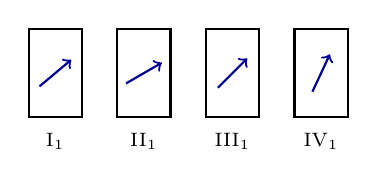
\begin{tikzpicture}[scale=0.75]
    \foreach \i/\ang/\lab in {
      0/40/I$_1$,
      1.5/30/II$_1$,
      3.0/45/III$_1$,
      4.5/65/IV$_1$}{
      \draw[thick] (\i,0) rectangle (\i+0.9,1.5);
      \pgfmathsetmacro\dx{0.35*cos(\ang)}
      \pgfmathsetmacro\dy{0.35*sin(\ang)}
      \draw[->,thick,blue!60!black]
        (\i+0.45-\dx, 0.75-\dy) -- (\i+0.45+\dx, 0.75+\dy);
      \node[below,font=\scriptsize] at (\i+0.45,-0.1) {\lab};
    }
  \end{tikzpicture}
  \caption{I$_1$—IV$_1$晶片快轴方向示意图}
  \label{fig:ext}
\end{figure}

\subsection{锥光干涉实验}

换用40×物镜，加入聚光镜与勃氏镜，调至正交偏光锥光状态。

\subsubsection{各类切片锥光干涉图比较}

\paragraph{z切晶片（垂直光轴切片）}

z切LN、Al$_2$O$_3$、薄石英、TeO$_2$及$\alpha$-BBO均在视域中央呈现\textbf{黑十字消光影}和\textbf{同心彩色干涉环}（白光光源）；旋转载物台时干涉图位置不变——为单轴晶垂直光轴切片的典型锥光干涉图（图\,\ref{fig:zcut}）。

各样品的异同：
\begin{itemize}
  \item \textbf{干涉环数目}（从多到少）：TeO$_2$（$\Delta n\approx0.14$）$>$z切LN（$\Delta n\approx0.086$）$>z$切$\alpha$-BBO（$\Delta n\approx0.012$）$>z$切薄石英/Al$_2$O$_3$（$\Delta n\approx0.009/0.008$），与双折射率大小对应；
  \item \textbf{黑臂宽度}：双折射率越低黑臂越宽（薄石英最宽，TeO$_2$最细）；
  \item z切\textbf{厚石英}（大方、小圆）干涉环比薄石英密集；且中心出现\textbf{埃利旋}，反映旋光性。
\end{itemize}

\paragraph{斜切晶片}

斜切薄LN、斜切厚LN和斜切TeO$_2$：黑十字交点（光轴露点）偏离视域中央；旋转载物台时，露点随之转动（方向相同），消光影始终平行上下偏光镜。斜切厚LN斜交角大，光轴露点超出视域范围，仅见弯曲黑臂。

\paragraph{平行光轴切片（x切）}

白云母与x切石英在0°位置出现\textbf{粗大模糊黑十字}；轻微转动载物台即分裂为两条双曲线沿光轴方向迅速移出视域（\textbf{瞬变干涉图}）；45°位置视域最亮，出现对称双曲线干涉带。

\subsubsection{光性正负鉴定}

对各z切晶片（厚石英除外）以两种方法鉴定光性，结果见表\,\ref{tab:sign}。

\begin{table}[H]
\centering
\caption{z切晶片光性正负鉴定结果}
\label{tab:sign}
\setlength{\tabcolsep}{3pt}
\begin{tabularx}{\columnwidth}{lYY}
\toprule
晶片 & 一级红插片法 & 石英楔子法 \\
\midrule
z切LN              & 负（$-$） & 负（$-$） \\
z切Al$_2$O$_3$     & 负（$-$） & 负（$-$） \\
z切薄石英           & 正（$+$） & 正（$+$） \\
$\alpha$-BBO       & 负（$-$） & 负（$-$） \\
TeO$_2$            & 无法判断  & 无法判断  \\
\bottomrule
\end{tabularx}
\end{table}

\textbf{判断依据（以z切薄石英为例）}：

\textit{一级红插片法}：插入后，\textbf{一、三象限}干涉色\textbf{升高}（$n_e$方向与插片慢轴平行，即$n_e$为慢轴，$n_e>n_o$），\textbf{二、四象限降低}，故判为\textbf{正光性}。

\textit{石英楔子法}：缓慢插入石英楔子时，\textbf{一、三象限}彩环\textbf{向内收缩}，\textbf{二、四象限向外扩张}（或二、四象限靠近黑十字处率先出现黑点），同样判为\textbf{正光性}，与前法吻合。

对z切LN（$n_e<n_o$）：一、三象限降低、二、四象限升高，彩环运动方向与石英相反，故为\textbf{负光性}。z切Al$_2$O$_3$和$\alpha$-BBO同理，均判为负光性。

TeO$_2$干涉环极密（双折射率约$0.14$），插入插片或楔子后颜色变化混乱，难以从四象限升降清晰判断，故光性\textbf{无法判断}。

\subsubsection{埃利旋与旋光性判断}

在锥光条件下，将z切厚石英（大方、小圆）及z切薄石英置于载物台，观察中心区域的埃利旋干涉图，结果见表\,\ref{tab:airy}。

\begin{table}[H]
\centering
\caption{石英旋光性判断结果}
\label{tab:airy}
\setlength{\tabcolsep}{4pt}
\begin{tabularx}{\columnwidth}{lY}
\toprule
样品 & 旋光方向 \\
\midrule
z切厚石英（大方） & \textbf{左旋}（卍形埃利旋） \\
z切厚石英（小圆） & \textbf{右旋}（卐形埃利旋） \\
z切薄石英         & 无法判断（环数少，图案不明显） \\
\bottomrule
\end{tabularx}
\end{table}

大方与小圆旋光方向相反：大方为\textbf{左旋}石英，小圆为\textbf{右旋}石英。厚晶片干涉环多，埃利旋清晰可辨；薄石英晶片干涉环少，中心旋转图案极不明显，\textbf{无法判断}旋光方向。

根据埃利旋理论，埃利旋的旋向取决于\textbf{下方晶片}的旋光方向：下方晶片左旋则观察到左旋卍形，下方晶片右旋则观察到右旋卐形。本实验中大方（左旋）观察到卍形图案，小圆（右旋）观察到卐形图案，与理论一致。

\subsubsection{标本样品观察（拓展）}

取\textbf{6号流纹岩}（Rhyolite）和\textbf{9号千枚岩}（Phyllite）切片，先在10×物镜下正交偏光观察，再换40×物镜进行锥光干涉实验。

\begin{itemize}
  \item \textbf{6号流纹岩}：正交偏光下可见多种矿物颗粒的不同干涉色（石英呈一、二级干涉色），具流动构造；40×锥光下石英颗粒可观测到清晰黑十字干涉图。
  \item \textbf{9号千枚岩}：云母类矿物定向排列，正交偏光下具有周期性消光；40×锥光干涉通过目镜观察清晰，但相机采集图像对比度较差，难以有效记录。
\end{itemize}

%%%%%%%%%%%%%%%%%%%%%%%%%%%%%%%%%%%%%%%%%%%%%%%%%%%%%%%%%%%%
\section{思考题}

\begin{enumerate}
  \item \textbf{光性正负鉴定两种方法的异同点，以及其适用的z切样品类别。}\\[0.3em]
  \textit{相同点}：两法均基于光程差补偿原理，通过四象限干涉色（或彩环）升降来判断$n_e$是快轴还是慢轴，进而确定正/负光性。
  \textit{不同点}：一级红插片产生固定$\Delta_0\approx\SI{530}{nm}$，插入后\textbf{静态}观察颜色变化，操作简便，适合干涉环数目较少的薄晶片（如薄石英、Al$_2$O$_3$）；石英楔子光程差连续变化，通过\textbf{动态}彩环移动或黑点出现位置判断，对干涉环较多的高双折射率样品（如z切LN、TeO$_2$）也能有效鉴定。两法均适用于垂直光轴（z切）单轴晶样品。

  \item \textbf{平行轴（x切）样品光轴和双折射光程差的判断注意事项。若光程差大于一级红或二级红？}\\[0.3em]
  需在\textbf{45°位置}（视域最亮）从视域中央干涉色查表估算$\Delta=d(n_e-n_o)$；光轴方向为干涉色从中心向边缘\textbf{降低}的两象限所指。若$\Delta>\SI{530}{nm}$（一级红）或$>\SI{1060}{nm}$（二级红），则需查较高级序的干涉色表；此时彩带密集、颜色辨别困难，可辅以石英楔子动态判断，或选用更薄的样品。

  \item \textbf{如何判断斜切样品光轴偏离方位；斜切厚LN为何观测不到彩色干涉条纹？}\\[0.3em]
  旋转载物台360°，锥光干涉图中光轴露点描出一个圆，圆心即镜轴位置；由露点相对视域中心的偏移方向即可确定光轴偏离方位。斜切厚LN（铌酸锂）不显彩色条纹，原因：LN双折射率极大（$\Delta n\approx0.086$）且晶片厚，各方向入射光的光程差均已超出高级序干涉色范围，不同波长光叠加趋于白色；等色曲线极密，超出分辨极限，故无法观察到彩色干涉条纹。

  \item \textbf{双折射率较低时黑十字粗，双折射率较高或晶片较厚时黑十字细乃至消失，如何解释？}\\[0.3em]
  黑臂宽度由PP/AA面附近能产生可分辨光程差所需的偏转角范围决定。双折射率低时，稍偏离PP/AA面的光需更大偏折角才能产生显著光程差，故消光影宽；双折射率高（或晶片厚）时，极小偏角即产生可分辨光程差，消光影极窄；双折射率极大时，消光影完全淹没于密集干涉彩环中而消失。

  \item \textbf{各向异性晶片在正交偏光下转动载物台一周，出现四次消光，如何解释？}\\[0.3em]
  由式（4-1-6），$I\propto\sin^2\!2\alpha$，消光条件为$\sin2\alpha=0$，即$\alpha=0^\circ,90^\circ,180^\circ,270^\circ$（OO与PP或AA平行）。转动360°时，OO与PP重合两次、与AA重合两次，共出现\textbf{四次消光}（每隔90°一次）；相邻消光之间有一次最亮（$\alpha=45^\circ,135^\circ,225^\circ,315^\circ$时$I$最大）。
\end{enumerate}

%%%%%%%%%%%%%%%%%%%%%%%%%%%%%%%%%%%%%%%%%%%%%%%%%%%%%%%%%%%%
\clearpage
\onecolumn
\section*{参考文献}

\begin{enumerate}[label={[\arabic*]}]
  \item 蒋民华. 晶体物理[M]. 济南：山东科学技术出版社, 1980.
  \item 季寿元, 王德滋. 晶体光学[M]. 北京：人民教育出版社, 1961.
  \item 金石琦. 晶体光学[M]. 北京：科学出版社, 1995.
  \item 郑裕芳, 李仲荣. 近代物理实验[M]. 广州：中山大学出版社, 1989.
  \item 孙业英. 光学显微分析[M]. 北京：清华大学出版社, 2003.
\end{enumerate}

\clearpage

\section{实验图片}
  
\begin{figure}[htbp]
  \centering
  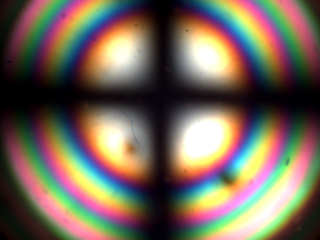
\includegraphics[width=0.45\columnwidth]{LN.png}
  \caption{z切LN锥光干涉图}
\end{figure}

\begin{figure}[htbp]
  \centering
  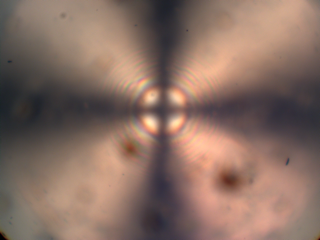
\includegraphics[width=0.45\columnwidth]{BBO.png}
  \caption{$\alpha$-BBO锥光干涉图}
\end{figure}

\begin{figure}[htbp]
  \centering
  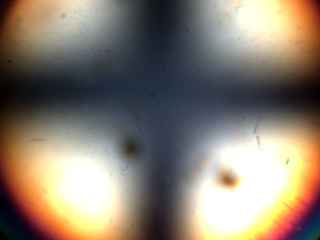
\includegraphics[width=0.45\columnwidth]{薄石英.png}
  \caption{薄石英锥光干涉图}
\end{figure}

\begin{figure}[htbp]
  \centering
  \includegraphics[width=0.45\columnwidth]{氧化铝.png}
  \caption{Al$_2$O$_3$锥光干涉图}
\end{figure}

\begin{figure}[htbp]
  \centering
  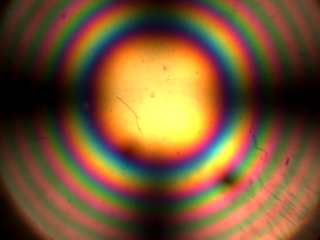
\includegraphics[width=0.45\columnwidth]{大方.png}
  \caption{厚石英（大方）锥光干涉图}
\end{figure}

\begin{figure}[htbp]
  \centering
  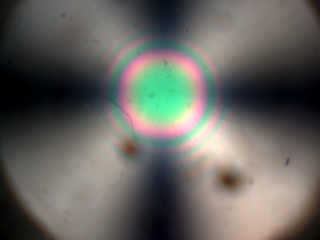
\includegraphics[width=0.45\columnwidth]{二氧化碲.png}
  \caption{TeO$_2$锥光干涉图}
\end{figure}

\begin{figure}[htbp]
  \centering
  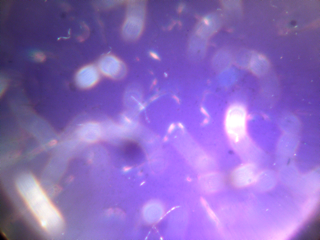
\includegraphics[width=0.45\columnwidth]{x切石英.png}
  \caption{x切石英锥光干涉图}
\end{figure}

\begin{figure}[htbp]
  \centering
  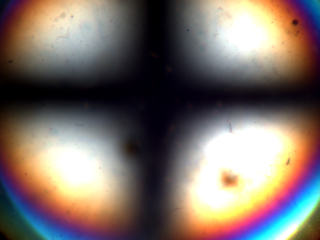
\includegraphics[width=0.45\columnwidth]{白云母1.png}
  \caption{x切白云母锥光干涉图（1）}
\end{figure}

\begin{figure}[htbp]
  \centering
  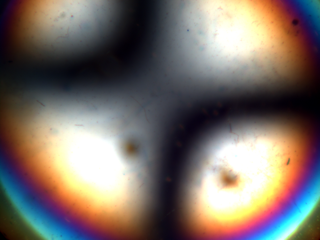
\includegraphics[width=0.45\columnwidth]{白云母2.png}
  \caption{x切白云母锥光干涉图（2）}
\end{figure}

\begin{figure}[htbp]
  \centering
  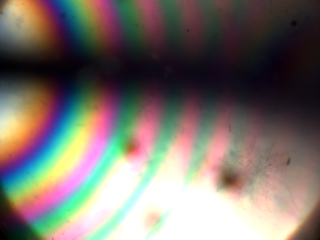
\includegraphics[width=0.45\columnwidth]{斜薄LN.png}
  \caption{斜切薄LN锥光干涉图}
\end{figure}

\begin{figure}[htbp]
  \centering
  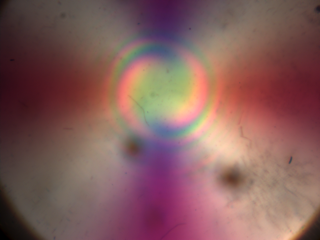
\includegraphics[width=0.45\columnwidth]{二氧化碲加红切片.png}
  \caption{TeO$_2$光性正负鉴定}
\end{figure}

\begin{figure}[htbp]
  \centering
  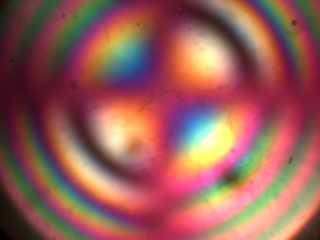
\includegraphics[width=0.45\columnwidth]{z切LN红插.png}
  \caption{z切LN光性正负鉴定}
\end{figure}

\begin{figure}[htbp]
  \centering
  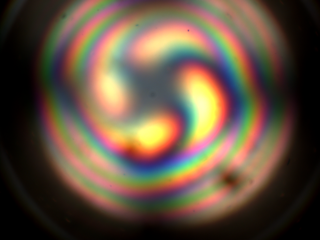
\includegraphics[width=0.45\columnwidth]{右旋.png}
  \caption{z切厚石英（小圆）旋光图}
\end{figure}

\begin{figure}[htbp]
  \centering
  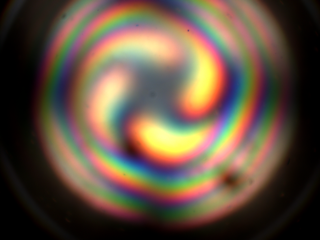
\includegraphics[width=0.45\columnwidth]{左旋.png}
  \caption{z切厚石英（大方）旋光图}
\end{figure}

\begin{figure}[htbp]
  \centering
  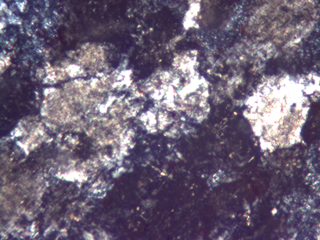
\includegraphics[width=0.45\columnwidth]{No6.png}
  \caption{流纹岩标本样品观察（正交偏光）}
\end{figure}

\begin{figure}[htbp]
  \centering
  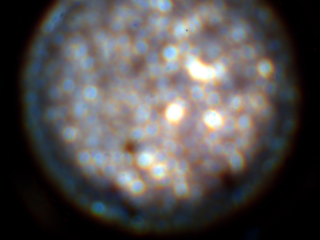
\includegraphics[width=0.45\columnwidth]{No6锥.png}
  \caption{流纹岩标本样品观察（锥光干涉）}
\end{figure}

\begin{figure}[htbp]
  \centering
  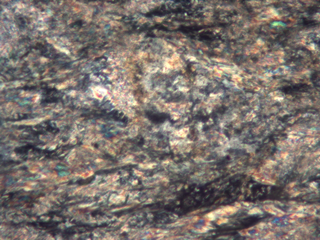
\includegraphics[width=0.45\columnwidth]{No9.png}
  \caption{千枚岩标本样品观察（正交偏光）}
\end{figure}

\begin{figure}[htbp]
  \centering
  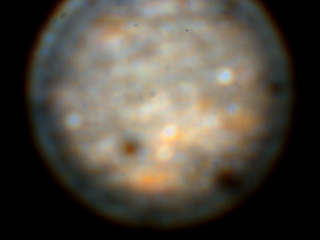
\includegraphics[width=0.45\columnwidth]{No9锥.png}
  \caption{千枚岩标本样品观察（锥光干涉）}
\end{figure}

\clearpage

\section{教师签名页}
  \begin{figure}[htbp]
  \centering
  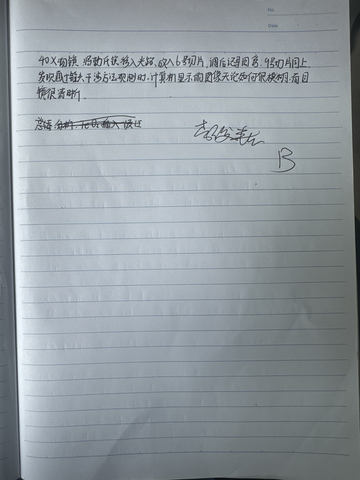
\includegraphics[scale=0.25]{影像.png}
  \caption{教师签名页（1）}
  \end{figure}

  \begin{figure}[htbp]
  \centering
  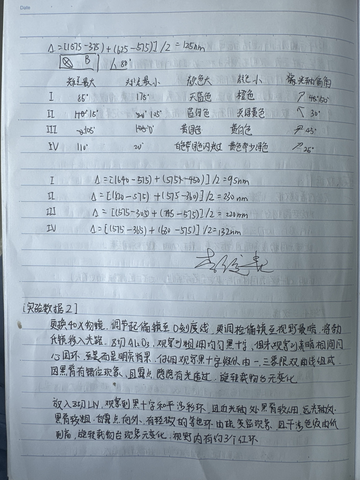
\includegraphics[scale=0.25]{影像 2.png}
  \caption{教师签名页（2）}
  \end{figure}


\end{document}
